\courseTime{Nov7 2022}
\section{复习}
\chat{%
总结前半学期的内容。

讲变分法。变分的原因是无法精确求解,用数值方法逼近。到这节课为止,之前的所有的体系(自由粒子、氢原子等等)都是可以精确求解的。现在复习以前的内容。

上半学期,由演绎和类比,得到量子力学的基本假设和框架。从原理上来说,本质上来说需要知道微观状态波函数。在一次量子化中可以由一次量子化求解薛定谔方程得到。因为哈密顿算符不含时,可分离得到静态薛定谔方程和含时部分。
}

这门课里所有的体系都是围绕定态薛定谔方程展开的,
\begin{align}
    \hat H \psi_i = E_i \psi_i.
\end{align}

\textbf{一维单粒子}
\begin{align}
    \hat H = \hat T + \hat V = -\frac{\hbar^2}{2m} \pdv[2]x + V(x). 
\end{align}

1. 自由粒子  $V(x) = 0$

2. 单侧无限深势阱
$V(x) = \begin{cases}
    0, \quad &x\in(0,l),\\
    +\infty, \quad &\text{其它},
\end{cases}$

3. 单侧半无限深势阱 $V(x)=\begin{cases}
    0, \quad &x\in(0,l), \\
    V, \quad &x\in[l,\infty), \\
    +\infty, \quad &x\in(-\infty, 0], 
\end{cases}$

4. 有限深势阱 $V(x) = \begin{cases}
    V, \quad &x \notin (0,l), \\
    0, \quad &x\in(0,l)
\end{cases}$

\chat{%
尽管这些模型很简单,也有它实际的意义。求解薛定谔方程,由品优波函数的假设,可以得到量子化条件。
}

5. 谐振子 $V(x) = \frac12 kx^2$,最复杂的一维单粒子模型,用幂级数求解。

我们又介绍了\textbf{二维单粒子}体系,与一维的不同在于其中的动能算符变成了二维,
\begin{align}
    \hat T = \hat T + \hat V = -\frac{\hbar^2}{2m} \left(\pdv[2]x + \pdv[2]y\right) + V(x,y). 
\end{align}
我们求解了

6. 粒子在环上的运动 $V(x,y) = \begin{cases}
    0, \quad &\sqrt{x^2 + y^2} = R, \\
    +\infty, \quad &\sqrt{x^2+y^2} \neq R,
\end{cases}$
求解它,要将笛卡尔坐标变换到极坐标 $(x,y) \rightarrow (r,\theta)$。

很快我们就到了\textbf{三维单粒子}体系,其动能算符也相应地变成三维的,
\begin{align}
    \hat T &= -\frac{\hbar^2}{2m} \left(\pdv[2]x + \pdv[2]y + \pdv[2]z\right) + V(x,y,z) \\
    &= -\frac{\hbar^2}{2m} \left(
        \hat\nabla_x^2 + \hat\nabla_y^2 + \hat\nabla_z^2 
    \right) = -\frac{\hbar^2}{2m} \hat\nabla^2, 
\end{align}

7. 球面 $V(x,y,z) = \begin{cases}
    0, \quad &\sqrt{x^2 + y^2 + z^2} = R, \\
    +\infty, \quad&\text{其它},
\end{cases}$
分离变量 $(x,y,z) \rightarrow (r,\theta,\varphi)$。

\textbf{三维两体},此时哈密顿量与两体有关,其中动能
\begin{align}
    \hat H = \hat T + \hat V = -\frac{\hbar^2}2 \sum_i \frac{1}{m_i} \hat\nabla_i^2 + \hat V(\vec r_1, \vec r_2, \cdots, \vec r_n),
\end{align}

8. 类氢离子,粒子感受到的是库仑力
\begin{align}
    V(\vec r_1, \vec r_2) = - \frac{Z_2 e^2}{|\vec r_1 - \vec r_2|},
\end{align}
想要求解它,(1) 将两体的运动分离成整体和相对运动 $(x_1, y_1, z_1, x_2, y_2, z_2) \rightarrow (X,Y,Z, x,y,z)$,质量变换 $(m_1, m_2) \rightarrow (M, m)$,哈密顿算符成为了
\begin{align}
    \hat H = - \frac{\hbar^2}{2M} \left(
        \pdv[2]X + \pdv[2]Y + \pdv[2]Z
    \right) - \frac{\hbar^2}{2\mu}  \left(
        \pdv[2]x + \pdv[2]y + \pdv[2]z
    \right) + V(\vec r), 
\end{align}
势函数成为了相对坐标的函数。(2) 复杂的地方在于其中的相对运动部分,
\begin{align}
    \hat H = -\frac{\hbar^2}{2\mu}  \left(
        \pdv[2]x + \pdv[2]y + \pdv[2]z
    \right) + V(\vec r), 
\end{align}
通过求解球面体系,我们知道要利用坐标变换,把哈密顿量变换到极坐标下 $(x,y,z) \rightarrow (r,\theta,\phi)$。

\chat{%
到底什么体系才是可以精确求解的?微分方程的通解是\boldtext{闭合表示}。数学中的闭合表示指可以通过有限次操作完成。前面可以精确求解的体系,都是可以由哈密顿量求出闭合解,进而求解。

对于三体的问题,氢分子能否精确求解?
}
\begin{figure}[tp]\centering
    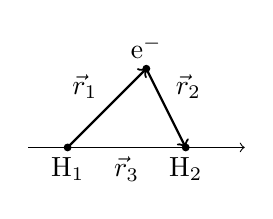
\begin{tikzpicture}[scale=0.5]
        \draw[->] (-3,0) -- (2.5, 0);
        \draw[->, thick] (-2,0) -- (0,2);
        \draw[->, thick] (0,2) -- (1,0);
        \node[below] at (-0.5,0) {$\vec r_3$};
        \node[above left] at (-1,1) {$\vec r_1$};
        \node[above right] at (0.5, 1) {$\vec r_2$};
    
        \fill (-2,0) circle (0.1);
        \fill (1,0) circle (0.1);
        \node[below] at (-2,0) {H$_1$};
        \node[below] at (1,0) {H$_2$};
        \fill (0,2) circle (0.1);
        \node[above] at (0,2) {e$^-$};
    \end{tikzpicture}
    \caption{氢分子示意图}
    \end{figure}

9. 氢分子,与氢原子唯一的不同是多了质子,
\begin{align}
    \hat H = - \frac{\hbar^2}{2m} \hat \nabla_1^2 - \frac{\hbar^2}{2m} \hat\nabla_2^2 - \frac{\hbar^2}{2m_\mathrm{e}} \hat \nabla_{\mathrm e}^2 + \frac{e^2}{r_3} - \frac{e^2}{r_1} - \frac{e^2}{r_2},
\end{align}
实际上它不可能通过坐标变换的方式分离三个变量。在 Born--Oppenheimer 近似下,将原子和电子运动分离开。

% 为什么不可以分离?三体是完全耦合的,数学上可以证明做不到。

分开原子核和电子的哈密顿量,其中电子的部分
\begin{align}
    \hat H = - \frac{\hbar^2}{2m} \hat\nabla_1^2 - \frac{\hbar^2}{2m} \hat\nabla_2^2 - \frac{\hbar^2}{2m_\mathrm{e}} \hat\nabla_{\mathrm{e}}^2 + \frac{e^2}{r_3} - \frac{e^2}{r_1} - \frac{e^2}{r_2},
\end{align}
三体全部两两耦合在一起,从数学角度不可能分离变量。

\suppInfo{波恩--奥本海默近似}{
因为原子核质量远大于电子质量,有三个数量级以上的差别,所以电子的运动会远远快于原子核。假设电子能迅速响应原子核位置的变化,或者假设原子核位置不动、将原子核坐标视为电子波函数的参数,从而分离原子核与电子的波函数,这称作 Born--Oppenheimer 近似。
}

分离之后,电子部分的哈密顿算符
\begin{align}
    \hat H = - \frac{\hbar^2}{2m_{\mathrm e}} \hat \nabla_\mathrm{e}^2 - \frac{e^2}{r_1} - \frac{e^2}{r_2},
\end{align}
它不能用简单的球谐函数求解,而是复杂的椭球函数。推荐文献 arXiv:quant-ph/0607081,给出了电子波函数的精确形式。

\begin{figure}[tp]\centering
    \begin{tikzpicture}[scale=0.7]
        \draw[->] (-1,0) -- (4,0);
        \draw[->] (0,-1) -- (0,3);
        
        \fill (0,0) circle (0.1);
        \fill (1,2) circle (0.1);
        \fill (3,1) circle (0.1);
    
        \draw[-Latex, thick] (0,0) -- (1,2);
        \draw[-Latex, thick] (0,0) -- (3,1);
        \draw[-Latex, thick] (1,2) -- (3,1);
    
        \node[below right] at (0,0) {He$_{(1)}$};
        \node[above] at (1,2) {e$^-_{(2)}$};
        \node[right] at (3,1) {e$^{-}_{(3)}$};
    
        \node[above right] at (2,1.5) {$\vec r_{23}$};
        \draw[->] (0.5,1) to [bend right] (-0.5, 2);
        \node[left] at (-0.5,2) {$\vec r_{12}$};
        \draw[->] (1.5,0.5) to [bend left] (3,-0.5);
        \node[below] at (3,-0.5) {$\vec r_{13}$};
    \end{tikzpicture}
    \caption{氦原子示意图}
    \end{figure}
10. 氦原子,它也是个三体的问题,此时有两个电子、一个原子核,哈密顿量
\begin{align}
    \hat H = -\frac{\hbar^2}{2m_1} \hat\nabla_1^2 -\frac{\hbar^2}{2m_{\mathrm{e}}} \hat\nabla_2^2 -\frac{\hbar^2}{2m_{\mathrm{e}}} \hat\nabla_3^2
    + \frac{e^2}{r_{23}} - 2\frac{e^2}{r_{12}} - 2\frac{e^2}{r_{13}},
\end{align}
毫无疑问不可以精确求解。在 BO 近似下,将原子核与电子分离,将电子的哈密顿量写成
\begin{align}
    \hat H_{\mathrm{e}} = -\frac{\hbar^2}{2m_{\mathrm{e}}} \hat\nabla_2^2 -\frac{\hbar^2}{2m_{\mathrm{e}}} \hat\nabla_3^2
    + \frac{e^2}{r_{23}} - 2\frac{e^2}{r_{12}} - 2\frac{e^2}{r_{13}},
\end{align}
这时候依然不可能精确求解,因为两个电子间的耦合 $r_{23}^{-1}$ 是必然存在的。

\chat{%
这就是本周(第十周,第 8 次课)的内容——变分法,用数值方法逼近体系的精确解。
}

\chapter{变分法}
\section{变分原理}
\begin{theorem}
    若已知体系哈密顿量 $\hat H$,如果 $\Phi$ 是任意一个满足此问题边界条件的归一化品优波函数,则有
    \begin{align}
        \langle \Phi | \hat H | \Phi \rangle \geqslant E_0, 
    \end{align}
    $E_0$ 为体系的基态真实能量。
\end{theorem}
\begin{proof}
    假设哈密顿量的本征算符有本征解,
    \begin{align}
        \hat H \phi_k = E_k \phi_k, \quad \langle \phi_k | \phi_j \rangle = \delta_{kj},
    \end{align}
    波函数可由本征函数展开,
    \begin{align}
        \Phi = \sum_k a_k \phi_k, 
    \end{align}
    %2022-11-07 08:42:44 Wenbin FAN @FDU
    重新展开成
    \begin{align}
        \langle \Phi | \hat H | \Phi \rangle 
        &= \big\langle \sum_k a_k^* \phi_k \big| \hat H \big| \sum_j a_j \phi_j \big\rangle \\
        &= \sum_k \sum_j a_k^* a_j \langle \phi_k | \hat H | \phi_j \rangle \\
        &= \sum_k \sum_j a_k^* a_j E_j \langle\phi_k | \phi_k \rangle \\
        &= \sum_k a_k^* a_k E_k \\
        &= \sum_k |a_k|^2 E_k,
    \end{align}
    因为 $E_0$ 是体系的基态能量,所以 $E_0 \leqslant E_k$。又因为 $|a_k|^2$ 总不为负,所以
    \begin{align}
        \langle\Phi | \hat H | \Phi \rangle = \sum_k |a_k|^2 E_k \geqslant \sum_k |a_k|^2 E_0 = E_0 \sum_k |a_k|^2, 
    \end{align}
    由归一化的假设可知
    \begin{align}
        1 = \langle\Phi | \Phi\rangle &= \Big\langle \sum_k a_k \phi_k \Big | \sum_j a_j \phi_j \Big\rangle \\
        &=\sum_k\sum_j a_k^* a_j \langle \phi_k|\phi_j \rangle \\
        &= \sum_k |a_k|^2,
    \end{align}
    系数的平方和为 1,那么变分原理可进一步写成
    \begin{align}
        \langle\Phi|\hat H|\Phi\rangle \geqslant E_0.  
    \end{align}
\end{proof}
若 $\{\Phi\}$ 并非归一化,$\langle\Phi|\Phi\rangle = N \neq 1$,构造 $\Phi' = \frac1{\sqrt N} \Phi$ 是归一化的波函数,
\begin{align}
    \langle \Phi' | \hat H | \Phi'  \rangle \geqslant E_0  \Rightarrow \frac1N \langle \Phi | \hat H | \Phi \rangle \geqslant E_0 \Rightarrow \frac{\langle \Phi' | \hat H | \Phi'  \rangle} {\langle \Phi' |  \Phi'  \rangle} \geqslant E_0,
\end{align}
则 $\{\Phi\}$ 称为尝试变分波函数 trail variation function,$\langle \Phi' | \hat H | \Phi'  \rangle$ 称为变分积分 variational integral。

下面要讲,如何利用变分原理求解能量。
\section{Rayleigh 变分法}
\chat{%
变分原理对尝试波函数没有任何限制,但我们很难构造所有可能的尝试波函数。所以,人们尝试构造一个波函数的参数空间,使得尝试波函数包含某些系数,通过调整这些参数来改变尝试波函数。
}

设 $\Phi=\Phi(c_1, c_2, c_3, \cdots, c_n)$,它的变分积分形式
\begin{align}
    \frac{\langle \Phi' | \hat H | \Phi'  \rangle} {\langle \Phi' |  \Phi'  \rangle} = f(c_1, c_2, \cdots, c_n),
\end{align}
对 $\{c_i\}$ 偏微分,求出 $f$ 的极值。当
\begin{align}
    \pdv{f}{c_1} = \pdv{f}{c_2} = \cdots = \pdv{f}{c_n} = 0
\end{align}
条件满足时,可以求出 $\{c_1^{(0)}, c_1^{(0)}, \cdots, c_1^{(0)}\}$,那么 $f(c_1^{(0)}, c_2^{(0)}, \cdots, c_n^{(0)})$ 就是对应于该尝试波函数最接近于 $E_0$ 的解。
% 上标的 $(0)$ 表示零级近似能量,
% 一级近似能量、零级近似波函数,
% 二级近似能量、一级近似波函数,
% 当年似乎是这么学的

\section{一维谐振子}
一维谐振子体系的哈密顿量为
\begin{align}
    \hat H &= - \frac{\hbar^2}{2m} \pdv[2]x + \frac12 kx^2, \quad k=m\omega^2, 
\end{align}
我们有尝试波函数 $\psi_0(\lambda) = N \ee^{-\lambda x^2}$,其中 $N$ 是归一化因子,$\lambda$ 是变分参数,下面求解变分积分,
\begin{align}
    f(\lambda) = \langle \psi_0 | \hat H | \psi_0 \rangle = N^2 \bigg\langle \ee^{-\lambda x^2} \bigg| -\frac{\hbar^2}{2m} \pdv[2]{x} + \frac12 k x^2 \bigg| \ee^{-\lambda x^2} \bigg\rangle,
\end{align}
令变分参数 $\lambda$ 的偏导为 0,得到了基态能量。第一步,
判断归一化因子,
\begin{align}
    \langle\psi_0 | \psi_0\rangle = 1 \Rightarrow N^2 \intinf \ee^{-2\lambda x^2} \dd x = 1, \label{eq:var_norm_step1}
\end{align}
\suppInfo{高斯积分}{有解析解,摘自 MathWorld\footnote{\url{https://mathworld.wolfram.com/GaussianIntegral.htm}。}
\begin{align}
    & \int_0^\infty \ee^{-ax^2} \dd x = \frac12 \sqrt{\pi}a, \\
    & \int_0^\infty x\,\ee^{-ax^2}\, \dd x = \frac1{2a},\\
    & \int_0^\infty x^2\,\ee^{-ax^2}\, \dd x = \frac1{4a}\sqrt{\frac{\pi}a},
\end{align}
}
所以上面归一化 \eqref{eq:var_norm_step1} 中的积分为
\begin{align}
    N^2 \sqrt{\frac{\pi}{2\lambda}} = 1 \Rightarrow N^2 = \sqrt{\frac{2\lambda}{\pi}}, 
\end{align}

第二部,求变分积分,先求两个偏导
\begin{align}
    &(\ee^{-\lambda x^2})' = -2\lambda x\,\ee^{-\lambda x^2}, \\
    &(\ee^{-\lambda x^2})'' = -2\lambda \,\ee^{-\lambda x^2} + 4 \lambda^2 x^2 \ee^{-\lambda x^2},
\end{align}
所以变分积分 $f(\lambda)$ 中的动能项为
\begin{align}
    &\phantom{=}{}\bigg\langle \ee^{-\lambda x^2} \bigg| -\frac{\hbar^2}{2m} \pdv[2]{x}  \bigg| \ee^{-\lambda x^2} \bigg\rangle \\
    &= \frac{\hbar^2\lambda}m \int_{-\infty}^{\infty} \ee^{-2\lambda x^2}\dd x - \frac{2\hbar^2\lambda^2}m \int_{-\infty}^{+\infty} \ee^{-2\lambda x^2} x^2 \dd x \\
    &= \frac{\hbar^2\lambda}m \sqrt{\frac{\pi}{2\lambda}} - 
    \frac{2\hbar^2\lambda^2}m \frac1{4\lambda} \sqrt{\frac{\pi}{2\lambda}} = \frac{\hbar^2\lambda}{2m} \sqrt{\frac{\pi}{2\lambda}},
\end{align}
势能项为
\begin{align}
    &\phantom{=}{}\bigg\langle \ee^{-\lambda x^2} \bigg|  \frac12 k x^2 \bigg| \ee^{-\lambda x^2} \bigg\rangle \\
    &= \frac12 k \intinf \ee^{-2\lambda x^2} x^2 \dd x \\
    &= \frac k2 \frac1{4\lambda} \sqrt{\frac{\pi}{2\lambda}} \\
    &= \frac{k}{8\lambda} \sqrt{\frac{\pi}{2\lambda}},
\end{align}
合并起来得到变分积分
\begin{align}
    f(\lambda) = \sqrt{\frac{2\lambda}{\pi}} \left(
        \frac{\hbar^2\lambda}{2m} \sqrt{\frac{\pi}{2\lambda}}
        + \frac{k}{8\lambda} \sqrt{\frac{\pi}{2\lambda}}
    \right) = \frac{\hbar^2\lambda}{2m} + \frac{k}{8\lambda},
\end{align}

第三步,对变分参数求导,
\begin{align}
    \pdv{f}{\lambda} = \frac{\hbar^2}{2m} - \frac{k}{8\lambda^2} = 0, \ \Rightarrow \ \lambda = \frac{\sqrt{mk}}{2\hbar} = \frac{m\omega}{2\hbar}, 
\end{align}
代回到变分积分中可得
\begin{align}
    f_\mathrm{min}(\lambda) = \frac{\hbar^2}{2m} \frac{m\omega}{2\hbar} + \frac k8 \frac{2\hbar}{m\omega} = \frac{\hbar\omega}2,
\end{align}
所以尝试波函数为
\begin{align}
    \psi_0 = N \exp\left(-\frac12 \frac{m\omega}{\hbar}x^2\right). 
\end{align}
由变分法得到了精确的能量和波函数。

\chat{%
所以说,只要采用正确的尝试波函数,总是可以由变分法来严格确定真实的波函数。实际上,真实的体系是复杂到无法构造尝试波函数的。

% 2022-11-07 09:30:00 Wenbin FAN @FDU
% 总是可以构造解决

变分法给了基态波函数最高的能量下限。通过尝试不同的尝试波函数来逼近求解。
}

\homework{\textbf{8.1} ~ 采用下列 Gaussian 函数作为氢原子的基态波函数,
\begin{align}
    \psi_0 = \exp\left(-\frac{\lambda r^2}{a_0^2}\right)
\end{align}
其中 $\lambda$ 是变分参数,$a_0$ 为 Bohr 半径,通过变分法给出能量表达式,并求出与真实氢原子基态能量的差别。
}

从上述求解可知,只要尝试波函数的形式合理,一定可通过调整变分参数使得尝试波函数足够接近精确解。换句话说,在完备的变分空间里,变分法等价于求解薛定谔方程。
\homework{
    \textbf{8.2} ~  从变分原理出发,推导定态薛定谔方程。
}

% 【】到了二维跟三维体系,【】给了习题 1,
% 2022-11-07 09:37:26 Wenbin FAN @FDU
% 【思路比较简单】怎么构造尝试波函数?

\chat{%
如果对氢原子感兴趣,可进一步思考:电子围绕着两个原子核运动,如果引入两个氢原子波函数的线性组合,是否能得到更准确的能量?下午会讲到。
}

\extraInfo{谐振子尝试波函数}{
    已知谐振子波函数的精确解,所以我们设尝试波函数的指数上为 $-\lambda x^2$,如果我们不知道是多少次方,假设是 $2k$ 次方,会是什么结果?此时尝试波函数写作
    \begin{align}
        \psi_0 = N^2 \ee^{-\lambda x^{2k}}, \quad N^2 = \frac12\frac{(2\lambda)^{\frac{1}{2 k}}}{\Gamma\!\left(1+\frac{1}{2 k}\right)},
    \end{align}
    变分积分为
    \begin{align}
        f(\lambda) = \frac12 N^2 \frac1{(2\lambda)^{\frac3{2k}} } \left[
            (2\lambda)^{2/k} \frac{k\hbar^2}{m} \Gamma\!\left(2-\frac1{2k}\right) + \frac{m\omega^2}k \Gamma\left(\frac{3}{2k}\right)
        \right],
    \end{align}
    求得极小值为
    \begin{align}
        f_{\mathrm{min}} = \omega\hbar k \sqrt{\Gamma\left(2-\frac1{2k}\right)\Gamma\left(\frac3{2k}\right)} \left[\Gamma\left(\frac1{2k}\right)\right]^{-1},
    \end{align}
    说这个点是极小值是因为二阶导大于 0。当 $k=1$ 时显然有 $f = \frac{\omega\hbar}2$,只有当 $k=1$ 时取得 $f_{\mathrm{min}}$ 的极小点,所以尝试波函数的指数上取 2 是最合适的。
}

\courseTime{下午 | 第8次课,第10周}
\chat{%
线上上课可能不容易控制时间,请见谅。

早上复习了从开课到现在的所有模型体系。我们在上午引入了氦原子,即使有 BO 近似,也无法精确求解,因为电子和电子之间有耦合项,因此又引入了变分法。
}
% 【】
\section{氦原子体系基态的变分处理}
氦原子包括一个原子核、两个电子,其电子部分的哈密顿量为
\begin{align}
    \hat H = -\frac{\hbar^2}{2m_{\mathrm{e}}} \hat\nabla_1^2 -\frac{\hbar^2}{2m_{\mathrm{e}}} \hat\nabla_2^2
    + \frac{e^2}{r_1} - 2\frac{e^2}{r_2} - 2\frac{e^2}{r_{12}},
\end{align}
最困难的是 $r_{12}^{-1}$ 的求解。如果暂不考虑电子间的相互作用,则
\begin{align}
    H_0 = -\frac{\hbar^2}{2m_{\mathrm{e}}} \hat\nabla_1^2 -\frac{\hbar^2}{2m_{\mathrm{e}}} \hat\nabla_2^2
    + \frac{e^2}{r_1} - 2\frac{e^2}{r_2}
\end{align}
此时电子1、电子2是可严格分离变量的,就相当于两个独立的类氢原子。基态的本征函数写作
% 2022-11-07 13:38:44 Wenbin FAN @FDU
% 本征函数可以精确求解
\begin{align}
    \psi(r_1, r_2) &= \psi_{100}(r_1) \psi_{100}(r_2) \\
    &= \frac1{\sqrt{\pi}} \left(\frac{Z}{a_0}\right)^{3/2} \exp\!\left(-\frac{Zr}{a_0}\right) \frac1{\sqrt\pi} \left(\frac{Z}{a_0}\right)^{3/2} 
    \exp\!\left(-\frac{Zr}{a_0}\right) \\
    &= \frac{Z^3}{\pi a_0^3} \exp\!\left[-\frac Z{a_0}(r_1 + r_2)\right],
\end{align}
\chat{%
现在毫无疑问,由于电子间相互作用,肯定跟无相互作用的波函数不一样,我们需要对它处理。如果要对它变分处理,如同早先对谐振子模型一样,需要构造尝试波函数的形状。尝试波函数的形状越合理,则能量越逼近真实情况。

我们可否通过无相互作用的基态波函数,得到构造尝试波函数的灵感呢?无相互作用的波函数中,其中有个 $Z$ 表示有效核电荷,如果有了电子-电子间的相互作用,第一个电子感受到第二个电子对于核电荷的屏蔽。}
于是,我们依照无相互作用的本征波函数,构造尝试波函数如下,
\begin{align}
    \psi_0(r_1, r_2; \lambda) = \psi_\lambda (r_1) \psi_\lambda(r_2) =  \frac{\lambda^3}{\pi a_0^3} \exp\!\left[-\frac \lambda{a_0}(r_1 + r_2)\right]. \label{eq:he_trial}
\end{align}
\chat{%
尝试波函数的构造和求解,是为了寻找更合适的 $Z$,使得能恰好描述屏蔽效应,进而得到具有物理意义的波函数。其中 $\lambda$ 是核电相互作用的有效电荷。
}

当我们构造了这样一个尝试波函数,按照 Rayleigh 的方法,第一步求出归一化系数,或者说验证是否归一,
\begin{align}
    \langle \psi_0 | \psi_0 \rangle &= \iint |\psi_0|^2 \,\dd\tau_1\,\dd\tau_2 \\
    &= \frac{\lambda^6}{\pi^2a_0^6} 
    \int \exp\!\left(-\frac{2\lambda}{a_0}r_1\right)\dd\tau_1 
    \int \exp\!\left(-\frac{2\lambda}{a_0}r_2\right)\dd\tau_2 
    \\
    &= \frac{\lambda^6}{\pi^2a_0^6} I^2,
\end{align}
接下来求其中的这个积分 $I$,在极坐标下更方便
\begin{align}
    I &= \int \exp\left(- \frac{2\lambda}{a_0} r\right) \dd\tau \\
    &= \int \exp\left(- \frac{2\lambda}{a_0} r\right) r^2 \sin\theta\,\dd r\,\dd\theta\,\dd\varphi \\
    &= \int_0^{+\infty} r^2 \exp\left(- \frac{2\lambda}{a_0} r\right) 
    \underbrace{\int_0^\pi \sin\theta\,\dd\theta \int_0^{2\pi} \dd\varphi}_{4\pi},
\end{align}
\chat{%
补充一个下面经常用到的积分公式,在徐光宪《量子化学:基本原理和从头计算法(中册)》(9.4.6),
\begin{align}
    \int_\rho^{+\infty} r^n \ee^{-ar} \dd r = a^{-(n+1)} \ee^{-a\rho} \ee^{-a\rho} \sum_{k=0}^n \frac{n!}{k!}(a\rho)^k,
\end{align}
}
利用该公式,继续求解积分,
\begin{align}
    I = 4\pi \times \left(\frac{2\lambda}{a_0}\right)^{-3} \frac{2!}{0!} 0^0 = 4\pi \frac{2a_0^3}{8\lambda^3} = \pi\left(\frac{a_0}{\lambda}\right)^3,
\end{align}
所以归一化积分为
\begin{align}
    \langle \psi_0 | \psi_0 \rangle = \frac{\lambda^6}{\pi^2a_0^6} \times \pi\left(\frac{a_0}{\lambda}\right)^3 \times \pi\left(\frac{a_0}{\lambda}\right)^3 = 1,
\end{align}
%2022-11-07 13:52:54 Wenbin FAN @FDU
验证了该尝试波函数是归一化的。
%2022-11-07 13:54:16 Wenbin FAN @FDU
所以,无论 $\lambda$ 取任何值,波函数都可以归一化的。

第二步,写出积分变量,
\begin{align}
    f(\lambda) = \langle \psi_0 | \hat H | \psi_0 \rangle,
\end{align}
因为哈密顿量
\begin{multline}
    \hat H 
    = -\frac{\hbar^2}{2m_\mathrm{e}} \left(\pdv[2]{x_1} + \pdv[2]{y_1} + \pdv[2]{z_1}\right) 
    - \frac{\hbar^2}{2m_\mathrm{e}} \left(\pdv[2]{x_2} + \pdv[2]{y_2} + \pdv[2]{z_2}\right) \\
    - \frac{2e^2}{r_1} - \frac{2e^2}{r_2} + \frac{e^2}{r_{12}},
\end{multline}
这里 Cartesian 坐标太复杂了,并不是说它不能求解。这里取一个简化的模式,拆分哈密顿量。怎么拆呢?按照尝试波函数,构造本征哈密顿量——类氢离子哈密顿量,哈密顿量应该写成
\begin{align}
    &\hat h_\lambda (r_1) = -\frac{\hbar^2}{2m} \hat\nabla_1^2 - \frac{\lambda e^2}{r_1} = -\frac{\hbar^2}{2m} \left(\hat\nabla_1^2 - \frac{2}{a_0}\frac{\lambda}{r_1}\right), \\
    &\hat h_{\lambda}(r_2) = -\frac{\hbar^2}{2m} \hat\nabla_2^2 - \frac{\lambda e^2}{r_2} = -\frac{\hbar^2}{2m} \left(\hat\nabla_2^2 - \frac{2}{a_0}\frac{\lambda}{r_2}\right), 
\end{align}
做了这样处理后,真实的哈密顿算符就可以写成
\begin{align}
    \hat H = \hat h_\lambda (r_1) + \hat h_\lambda (r_2)
    + \frac{\hbar^2}{ma_0} 
    \left(
        \frac{\lambda-2}{r_1} + 
        \frac{\lambda-2}{r_2} + 
        \frac1{r_{12}}
    \right),
\end{align}
\chat{%
我们把尝试波函数拆成了,其本征函数,加上其与真实波函数的差别。有什么好处?$\hat h$ 可精确求解,避免了动能算符的偏导,剩下的只是势能算符的积分,就比较好处理。
}

为何说 $\hat h$ 是尝试波函数的本征函数,因为
\begin{align}
    \langle \psi_0 | \hat h | \psi_0 \rangle = - \lambda^2 \frac{\hbar^2}{2m a_0^2} = \lambda^2 E_{\text{H}}. 
\end{align}
无论 $\lambda$ 取任何值,尝试波函数 \eqref{eq:he_trial}
% \begin{align}
%     \psi_0(r_1, r_2, \lambda) = \frac{\lambda^2}{\pi a_0^3} [][]
% \end{align}
都是 $\hat h_1 + \hat h_2$ 的本征函数。

有了这种拆分,期望值可分成三个部分,对每一部分求解。

第一部分,本征函数,
\begin{align}
    &\phantom{{}={}} \langle \psi_0 | \hat h_\lambda (r_1) + \hat h_\lambda (r_2) | \psi_0 \rangle
    \\
    &=
    \underbrace{\langle \psi_\lambda(r_1) | \hat h_\lambda (r_1) | \psi_\lambda(r_1) \rangle}_{\text{类氢离子基态能量}} 
    \underbrace{\langle \psi_\lambda(r_2) | \psi_\lambda (r_2) \rangle}_{\text{归一化}} \notag\\
    &\phantom{{}={}}+ \langle \psi_\lambda(r_2) | \hat h_\lambda (r_2) | \psi_\lambda(r_2) \rangle  \langle \psi_\lambda(r_1) | \psi_\lambda (r_1) \rangle
    \\
    &= 2 \left(- \frac{\hbar^2\lambda^2}{2ma_0^2}\right) = -\frac{\hbar^2\lambda^2}{ma_0^2}
\end{align}
第二部分,
\begin{align}
    &\phantom{{}={}}\Big\langle \psi_0 \Big | \frac{\hbar^2}{ma_0} \frac{\lambda-2}{r_1} \Big | \psi_0 \Big\rangle\\
    &=\frac{\hbar^2}{ma_0} \langle \psi_\lambda (r_2) | \psi_\lambda (r_2) \rangle \bigg\langle \psi_\lambda(r_1) \bigg| \frac{\lambda-2}{r_1} \bigg| \psi_\lambda(r_2) \bigg\rangle \\
    &=\frac{\hbar^2}{ma_0} (\lambda-2) \bigg\langle \psi_\lambda(r_1) \bigg| \frac{1}{r_1} \bigg| \psi_\lambda(r_2) \bigg\rangle
\end{align}
其中
\begin{align}
    &\phantom{{}={}}\Big\langle \psi_\lambda \Big| \frac1{r} \Big| \psi_\lambda \Big\rangle \\
    &= \frac{\lambda^3}{\pi a_0^3} \int_0^{+\infty} \exp\left(- \frac{2\lambda r}{a_0}\right) \frac1{r} r^2 \dd r \int_0^\pi \sin\theta\dd\theta \int_0^{2\pi} \dd\varphi \\
    &= \frac{4\lambda^3}{a_0^3} \int_0^\infty \exp\!\left(-\frac{2\lambda r}{a_0}\right)r \,\dd r \\
    &= \frac{4\lambda^3}{a_0^3} \left(\frac{a_0}{2\lambda}\right)^2 = \frac{\lambda}{a_0}, 
\end{align}
所以第二部分积分得到
\begin{align}
    \Big\langle \psi_0 \Big | \frac{\hbar^2}{ma_0} \frac{\lambda-2}{r_1} \Big | \psi_0 \Big\rangle
    =\frac{\lambda(\lambda-2)\hbar^2}{ma_0}. 
\end{align}
第三部分跟第二部分一样。所以组合起来各部分,得到变分积分为
\begin{align}
    f(\lambda) &= -\frac{\hbar^2\lambda^2}{ma_0^2} + 
    \frac{2\lambda(\lambda-2)\hbar^2}{ma_0} + \frac{\hbar^2}{ma_0} \bigg \langle \psi_0 \bigg | \frac1{r_{12}} \bigg | \psi_0 \bigg\rangle 
    \\
    &= \frac{\lambda^2 - 4\lambda}{ma_0}\hbar^2 + \frac{\hbar^2}{ma_0} \bigg \langle \psi_0 \bigg | \frac1{r_{12}} \bigg | \psi_0 \bigg\rangle
\end{align}
那么困难就是在如何求后面这个积分。
\courseTime{4th, week8, Nov 07}
% 第四节课
\subsection{耦合项的积分}
耦合项 $r_{12}^{-1}$ 的积分是用变分法求解氦原子的核心 hardcore 难点,该项的积分为
\begin{multline}
    \bigg\langle \psi_0 \bigg| \frac1{r_{12}} \bigg| \psi_0 \bigg\rangle = \frac1{\pi^2} \left(\frac{\lambda}{a_0}\right)^6 
    \underbrace{\int_0^{+\infty} r_1^2 \dd r_1 \int_0^\pi\sin\theta_1 \dd\theta_1 \int_0^{2\pi} \dd\varphi_1}_{\text{第一个电子}} \\ \times
    \underbrace{\int_0^{+\infty} r_2^2 \dd r_2 \int_0^\pi\sin\theta_2 \dd\theta_2 \int_0^{2\pi} \dd\varphi_2}_{\text{第二个电子}} 
    \frac1{r_{12}} \exp\left[-\frac{2\lambda}{a_0}(r_1 + r_2)\right], 
\end{multline}
困难在于,这是关于两个电子的积分,不幸的是后面有耦合项。

\begin{figure}\centering
    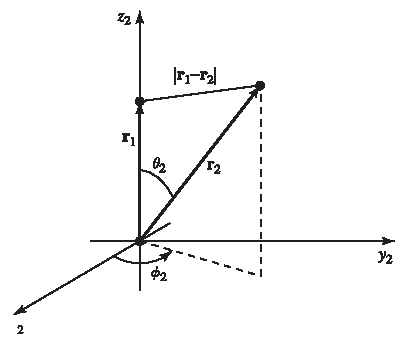
\includegraphics[height=6cm]{fig/r2_integral.pdf}
    \caption{耦合积分中的坐标选择,本图来自 Griffth 书的图 7.4}
    \label{fig:coupled_r2}
\end{figure}
\chat{%
注意到,这两个电子的坐标都是自由的。我们尝试\textbf{分开求解},分而治之,把 $r_1$ 看成是固定的,能否积掉 $r_2$?利用这个假设,参照图 \ref{fig:coupled_r2} 的定义,}
那么
\begin{align}
    r_12 = |r_1 - r_2| = \sqrt{r_1^2 + r_2^2 - 2r_1 r_2 \cos\theta_2}. 
\end{align}
先求解其中 $\theta_2$ 的积分(下面 $I_2$ 的 2 仅用来标记积分内容,无特殊含义,后面的 $I_3$ 等同理),
\begin{align}
    I_2&=\int_0^\pi \sin\theta_2 \, \frac1{r_{12}} \dd\theta_2 \\
    &=\int_0^\pi \frac{\sin\theta_2}{\sqrt{r_1^2 + r_2^2 - 2r_1 r_2 \cos\theta_2}}\dd\theta_2
\end{align}
设 $x = -\cos\theta_2$,则 $\dd x = \sin\theta_2\dd\theta_2$,代回上式,
\begin{align}
    I_2 &= \int_{-1}^1 \frac{\dd x}{\sqrt{r_1^2 + r_2^2 - 2r_1 r_2 x }}
\end{align}
\chat{%
利用积分公式
\begin{align}
    \int \frac{\dd x}{\sqrt{a+bx}} = \frac2b \sqrt{a+bx}
\end{align}
}
继续求解
\begin{align}
    I_2&= \frac{2}{2r_1r_2} \left(
        \sqrt{r_1^2 + r_2^2 + 2r_1r_2} - \sqrt{r_1^2+r_2^2 - 2r_1r_2}
    \right) \\
    &= \frac1{r_1r_2} \left(
        r_1 + r_2 - |r_1 - r_2|
    \right)\\
    &= \frac1{r_1r_2} \times \begin{cases}
        2r_2, \quad & r_1 \geqslant r_2, \\
        2r_1, \quad & r_1 < r_2,
    \end{cases} 
    = \begin{cases}
        \frac{2}{r_1}, \quad r_1 \geqslant r_2, \\
        \frac{2}{r_2}, \quad r_1 < r_2, 
    \end{cases}
    \\
    &= \frac2{\max\{r_1, r_2\}},
\end{align}
再求其余跟 $r_2$ 相关的部分
\begin{align}
    I_3{}& \int_0^\infty r_2^2 \dd r_2 \int_0^\pi \sin\theta_2 \dd\theta_2 \int_0^{2\pi}\dd\varphi_2 \frac1{r_{12}}
    \exp\left[-\frac{2\lambda}{a_0}(r_1 + r_2)\right] 
    \\
    ={}& \int_0^\infty r_2^2 \dd r_2 \exp\left[
        -\frac{2\lambda(r_1 + r_2)}{a_0}
    \right] \frac{2}{\max\{r_1, r_2\}} 
    \int_0^{2\pi} \dd\varphi_2 \\
    ={}& 4\pi \exp\left(-\frac{2\lambda r_1}{a_0}\right) 
    \int_0^{+\infty} r_2^2 \exp\!\left(-\frac{2\lambda}{a_0}r_2\right) \frac1{\max\{r_1, r_2\}} \dd r_2, 
\end{align}
其中的 max 相当于分段函数,分开积分
\begin{align}
    I_3 &= 4\pi \exp\left(
        -\frac{2\lambda r_1}{a_0}\right)
        \left[
            \int_0^{r_1} r_2^2 \exp\left(- \frac{2\lambda}{a_0}r_2\right) \frac1{r_1} + \int_{r_1}^{r_2} \exp\!\left(-\frac{2\lambda}{a_0}r_2\right) \frac1{r_2} \dd r_2
        \right]
\end{align}
\chat{%
利用已知积分
\begin{align}
    &\int r \ee^{-ar} \dd r= - \frac{ra + 1}{a^2} \ee^{-a r}, \\
    &\int r^2 \ee^{-ar}\dd r = - \frac{r^2a^2 + 2ra + 2}{a^3} \ee^{-ar},
\end{align}
}
继续求解积分,
\begin{align}
    I_3 &= 4\pi \exp\left(- \frac{2\lambda}{a_0}r_1\right) 
    \Bigg[
        \frac 1{r_1} - \frac{r_1^2 \left(\frac{2\lambda}{a_0}\right)^2 + 2 \frac{2\lambda}{a_0} r_1 + 2}{\left(\frac{2\lambda}{a_0}\right)^3} \exp\left(-\frac{2\lambda}{a_0}r_1\right) \notag\\
    &\phantom{=} + \frac{2}{\left(\frac{2\lambda}{a_0}\right)^3} + \frac{r_1 \left(\frac{2\lambda}{a_0}\right) + 1}{\left(\frac{2\lambda}{a_0}\right)^2} \exp\!\left(-\frac{2\lambda}{a_0}r_1\right)\Bigg]\\
    &=\frac{4\pi a_0^3}{8\lambda^3} \frac1{r_1} \exp\!\left(-\frac{2\lambda}{a_0}r_1\right) 
    \left[
        -\left(\frac{2\lambda}{a_0}r_1 + 2\right) \exp\!\left(-\frac{2\lambda}{a_0}r_1\right) + 2
    \right] \\
    &=\frac{\pi a_0^3}{\lambda^3} \frac1{r_1} \left[
        \exp\left(-\frac{2\lambda}{a_0}r_1\right) - \left(1+\frac{\lambda}{a_0}r_1\right) \exp\left(-\frac{4\lambda}{a_0}r_1\right)
    \right]
\end{align}
求解完了 $r_2$ 相关的部分,把这个积分代回 $r_{12}$ 的积分中去,有
\begin{align}
    &\int_0^{+\infty} r_1^2 \dd r_1 \frac{\pi a_0^3}{\lambda^3} \frac1{r_1}  
    % \notag \\ &\quad \times
    \left[
        \exp\!\left(-\frac{2\lambda}{a_0}r_1\right) - \left(1+\frac{\lambda}{a_0}r_1\right) \exp\left(-\frac{4\lambda}{a_0}r_1\right)
    \right] \notag \\
    &\quad \times \int_0^\pi \sin\theta_1 \dd\theta_1
    \int_0^{2\pi} \dd\varphi_1 \\
    =& \frac{4\pi^2 a_0^3}{\lambda^3} \int_0^{+\infty} r_1 
    \left[
        \exp\!\left(-\frac{2\lambda}{a_0} r_1\right) - \exp\!\left(-\frac{4\lambda}{a_0}r_1\right) - 
        \frac{\lambda}{a_0} r_1 \exp\!\left(-\frac{4\lambda}{a_0} r_1\right)
    \right] \dd r_1 \notag
    \\
    =& \frac58 \frac{\pi a_0^5}{\lambda^5}
\end{align}
最终有 $r_{12}^{-1}$ 部分的积分为
\begin{align}
    \bigg\langle \psi_0 \bigg| \frac1{r_{12}} \bigg| \psi_0 \bigg\rangle = \frac1{\pi^2}\left(\frac{\lambda}{a_0}\right)^6 \times \frac58 \frac{\pi a_0^5}{\lambda^5} = \frac58 \frac{\lambda}{a_0},
\end{align}
则
\begin{align}
    f(\lambda) &= \frac{\lambda^2 - 4\lambda}{ma_0}\hbar^2 + \frac{\hbar^2}{ma_0} \frac58 \frac{\lambda}{a_0} \\
    &= \frac{\hbar^2}{ma_0} \left(\lambda^2 - \frac{27}8 \lambda\right), 
\end{align}
对变分参数求偏导可得
\begin{align}
    \pdv{f(\lambda)}{\lambda} = 0 \ \Rightarrow \ \lambda = \frac{27}{16} = \num{1.6875}.
\end{align}
由于电子的相互排斥,相当于对有效核电荷起到了屏蔽效应,使得电子感受到的平均核电荷有相互吸引的部分。此时基态能量为
\begin{align}
    E_0 \approx \langle \psi_0|\hat H | \psi_0\rangle = \frac{\hbar^2}{ma_0} \left(\lambda^2 - \frac{27}8 \lambda\right) \approx \num{-2.848} \frac{\hbar^2}{ma_0} \geqslant E_0 = \num{-2.904} \frac{\hbar^2}{ma_0}. 
\end{align}
由参数 $\lambda$ 便可以给出氦原子基态能量的近似值,我们看到确实变分能量高于真实能量。

% 2022-11-07 15:03:15 Wenbin FAN @FDU
\chat{%
变分法不能保证,构造出的尝试波函数空间一定涵盖真实的波函数,如果能够涵盖基态波函数,如谐振子模型,但绝大多数体系是不可能的,如氦原子是最简单的一个做不到的例子。虽然我们做不到精确,但是我们可以不断逼近。
}

有没有办法可以更好地逼近?
\chat{%
回头来审视最初的设定,如果两个例子感受到的有效电荷不一样,是否能更精确地求解?
}
\homework{\textbf{8.3} ~  请用下述波函数作为尝试波函数,
\begin{align}
    \Phi_0 = N \left(
        \ee^{-\lambda_1 r_1/a_0} \ee^{-\lambda_1 r_2} + 
        \ee^{-\lambda_2 r_1/a_0} \ee^{-\lambda_2 r_2}
    \right),
\end{align}
变分积分为 $f(\lambda_1, \lambda_2) = \langle \Phi_0 | \hat H | \Phi_0 \rangle$,对于 BO 近似下的氦原子电子基态能量进行变分,能量约为 $\num{-2.88}\frac{\hbar^2}{ma_0}$,参考 Eckart, C. (1930). The theory and calculation of screening constants. \emph{Physical Review}, \emph{36}(5), 878. DOI: 10.1103/PhysRev.36.878 。
}

%2022-11-07 15:09:03 Wenbin FAN @FDU
能否得到激发态能量?
\chat{%
也可以的,通过正交的方式得到,具体拓展下节课线下再讲。
}